\section{SHMAC}

SHMAC is a hardware prototype of a Single-ISA Heterogeneous MAny-core Computer
\cite{shmacsliedes, shmacwebpage, Rusten567042}. It is an ongoing research
project within the Energy Efficient Computing Systems (EECS) research area at
the Department of Computer and Information Science, and Department of
Electronics and Telecommunications at NTNU. The SHMAC project is driven by the
\textit{dark silicon effect}: as transistors become smaller, only parts of a
chip can be powered simultaneously \cite{esmaeilzadeh2011dark}. SHMAC implements
two main strategies to mitigate the dark silicon effect, heterogeneity and
specialization.

\begin{figure}
    \centering
    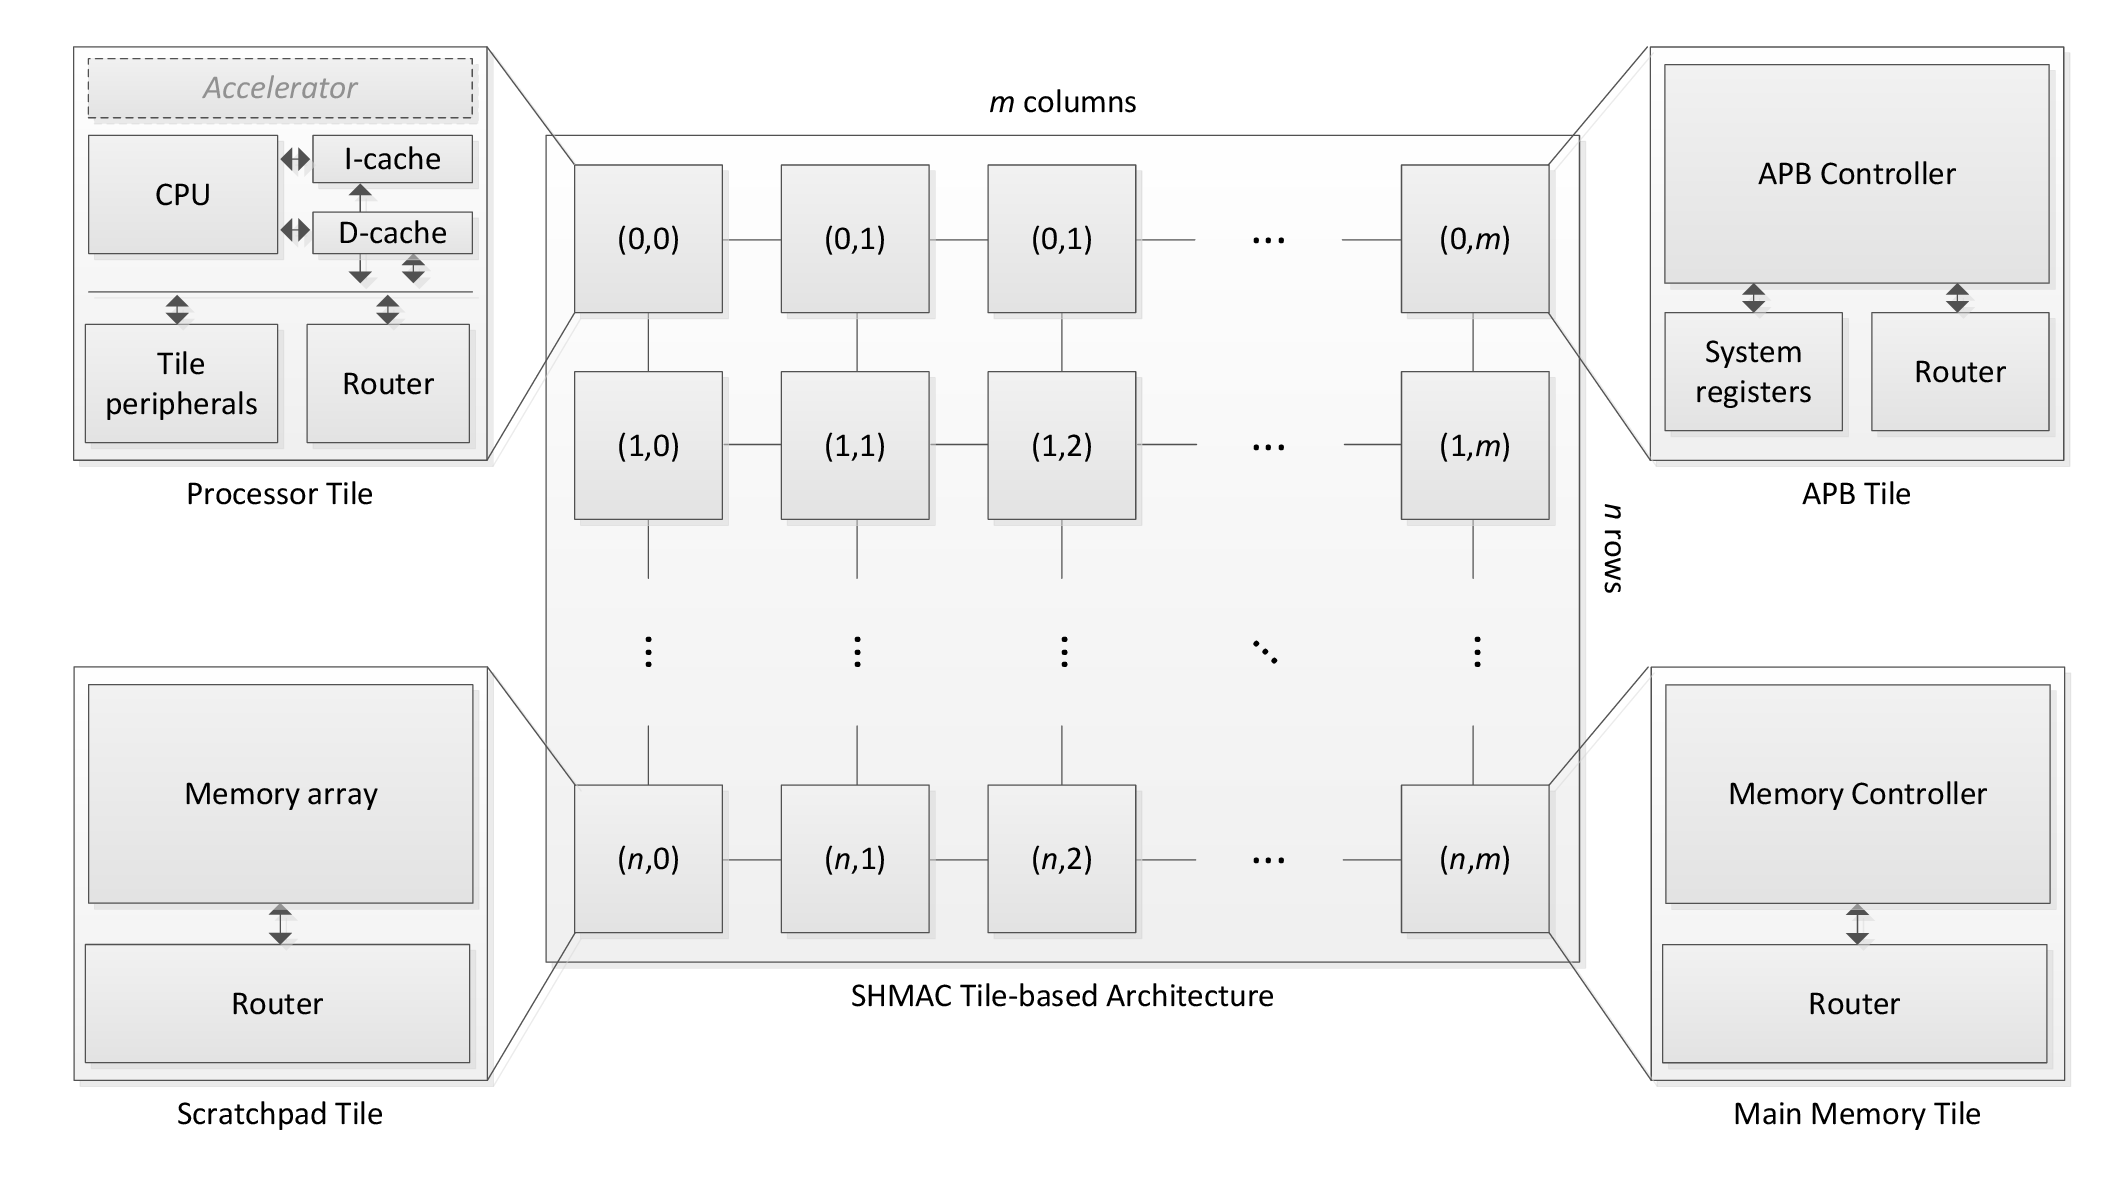
\includegraphics[width=1.0\textwidth]{figs/shmac-high-level2.png}
    \caption{The SHMAC architecture. The figure shows how different kind of
        tiles are combined together and form a complete architecture. From
        \cite{shmacwebpage}.}
    \label{fig:shmac}
\end{figure}

The SHMAC architecture is tile-based. Processing elements are laid out in a
rectangular grid with connections to their nearest neighbor, as depicted in
\autoref{fig:shmac}. A router device present in all SHMAC tiles handles
communication and data flow between tiles. In SHMAC, different kinds of
specialized tiles/accelerators can be composed as desired, to form a computer
tailored to the application. With the ability to evaluate different tiles with
respect to energy and performance, the most advantageous core composition can be
chosen.
